%!TEX root=../robocert.tex
\begin{figure}[htb]
	\centering
	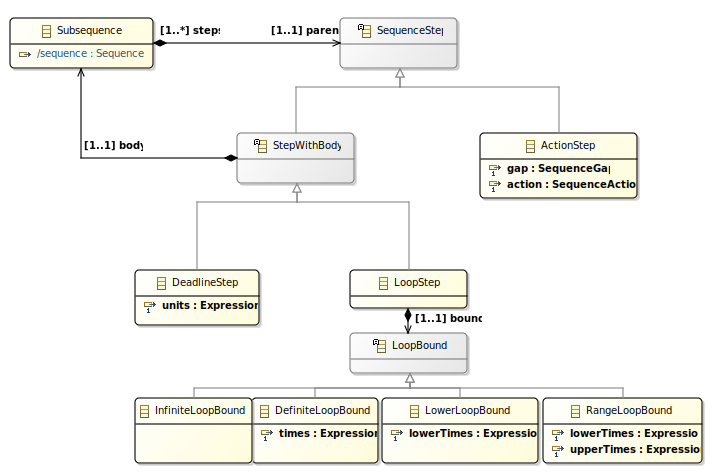
\includegraphics[width=0.7\textwidth]{diagrams/Steps}
	\caption{Class diagram for the part of the \langname{} metamodel dealing with steps.}
	\label{fig:metamodel-steps}
\end{figure}

\noindent
Steps (\msequencestep) are elements of
\msubsequence s.  They represent both communications and control flow, and
can themselves contain \msubsequence s.  There are three types of
step:

\begin{itemize}
\item \mdeadlinestep{} (\cref{ssec:metamodel-steps-deadline});
\item \mloopstep{} (\cref{ssec:metamodel-steps-loop});
\item \mactionstep{} (\cref{ssec:metamodel-steps-action});
\end{itemize}

\Cref{fig:metamodel-actions} depicts the part of the metamodel concerning
sequence steps.

\subsection{\mdeadlinestep}\label{ssec:metamodel-steps-deadline}

A \mdeadlinestep{} asserts that a \msubsequence{} terminates within
a given number of time units.  \todo{is this definitely a deadline?}
It takes a name (currently only
used in the graphical notation), and an expression that must
evaluate to a natural number of time units.

\begin{remark}
To specify that all actions in a \msubsequence{} must occur
immediately, use a deadline of \(0\).
\end{remark}

\begin{figure}[H]
\begin{subfigure}[t]{\egtextwidth}
\begin{lstlisting}[style=Example]
deadline T : within 3 units {
    ->op O1()
}
\end{lstlisting}
\end{subfigure}
\hfill
\begin{subfigure}[t]{\eggraphicalwidth}
  \gsecaption
  \centering
  \begin{tikzpicture}
\matrix[diagram]{
  \node[rcmodule](mstart) {\egtarget}; & \node[world](wstart) {\egworld}; \\
  & \coordinate(wds); & \\
  \coordinate(mo); & \coordinate(wo); & \\
  \coordinate(mde); & \coordinate(wde); \\
};
\draw[lifeline] (mstart) -- (mo) -- (mde);
\draw[lifeline] (wstart) -- (wds) -- (wo) -- (wde);
\gdeadline{wds}{wde}{T}{3}
\draw (mo) edge[oarrow, "O1()"] (wo);
  \end{tikzpicture}
\end{subfigure}
\end{figure}


\subsection{\mloopstep}\label{ssec:metamodel-steps-loop}

% Shorthand for introducing the loop action diagram matrix.
\newcommand{\egloopmatrix}{
  \node[rcmodule](mstart) {\egtarget}; \pgfmatrixnextcell \node[world](wstart) {\egworld}; \\
  \coordinate(mls); \pgfmatrixnextcell \coordinate(wls); \\
  \coordinate(mo); \pgfmatrixnextcell \coordinate(wo); \\
  \coordinate(mle); \pgfmatrixnextcell \coordinate(wle); \\
}
% Draws the entire loop diagram with the given loop bound header.
\newcommand{\egloopdiagram}[1]{
  \matrix[diagram]{\egloopmatrix};
  \draw[lifeline] (mstart) -- (mls) -- (mo) -- (mle);
  \draw[lifeline] (wstart) -- (wls) -- (wo) -- (wle);
  \draw (mo) edge[oarrow, "O1()"] (wo);
  \gloop{mls}{wls}{mle}{wle}{L}{#1}
}

A \mloopstep{} is a named loop over a \msubsequence{} of steps.
The number of times a \mloopstep{} will iterate \todo{breaking forthcoming}
depends on its attached \mloopbound{}.  Each bound is in terms of
\mexpression{}s that are evaluated \emph{only once}, before the execution
of the loop.

\paragraph{\minfiniteloopbound}
A \minfiniteloopbound{} states that the loop executes an infinite
number of times.

\begin{figure}[H]
\begin{subfigure}[t]{\egtextwidth}
\begin{lstlisting}[style=Example]
loop L : forever { // or 'loop L {'
    ->op O1()
}
\end{lstlisting}
\end{subfigure}
\hfill
\begin{subfigure}[t]{\eggraphicalwidth}
  \gsecaption
  \centering
  \begin{tikzpicture}
    \egloopdiagram{\gloopinfinite}
  \end{tikzpicture}
\end{subfigure}
\end{figure}

\paragraph{\mdefiniteloopbound}
A \mdefiniteloopbound{} states that the loop executes exactly the
number of times given in the bound.

\begin{figure}[H]
\begin{subfigure}[t]{\egtextwidth}
\begin{lstlisting}[style=Example]
loop L : exactly 4 times {
    ->op O1()
}
\end{lstlisting}
\end{subfigure}
\hfill
\begin{subfigure}[t]{\eggraphicalwidth}
  \gsecaption
  \centering
  \begin{tikzpicture}
    \egloopdiagram{\gloopdefinite{4}}
  \end{tikzpicture}
\end{subfigure}
\end{figure}

\paragraph{\mlowerloopbound}
A \mlowerloopbound{} states that the loop executes at least the
number of times given in the bound, but may nondeterministically
choose to execute any number of times in addition.

\begin{figure}[h!]
\begin{subfigure}[t]{\egtextwidth}
\begin{lstlisting}[style=Example]
loop L : at least 5 times {
    ->op O1()
}
\end{lstlisting}
\end{subfigure}
\hfill
\begin{subfigure}[t]{\eggraphicalwidth}
  \gsecaption
  \centering
  \begin{tikzpicture}
    \egloopdiagram{\glooplower{5}}
  \end{tikzpicture}
\end{subfigure}
\end{figure}

\paragraph{\mrangeloopbound}
A \mrangeloopbound{} behaves as a \mlowerloopbound, but states that
the loop will not execute any more times than the given upper bound.
Note that if the bounds are the same, the semantics is equivalent
to that of a \mdefiniteloopbound{}.

\begin{figure}[H]
\begin{subfigure}[t]{\egtextwidth}
\begin{lstlisting}[style=Example]
loop L : between 3 and 6 times {
    ->op O1()
}
\end{lstlisting}
\end{subfigure}
\hfill
\begin{subfigure}[t]{\eggraphicalwidth}
  \gsecaption
  \centering
  \begin{tikzpicture}
    \egloopdiagram{\glooprange{3}{6}}
  \end{tikzpicture}
\end{subfigure}
\end{figure}

\subsection{\mactionstep}\label{ssec:metamodel-steps-action}

A \mactionstep{} contains a specification of a
\msequenceaction{} (\cref{sec:metamodel-actions}), as well as
a \msequencegap{} (\cref{ssec:metamodel-steps-gaps})
capturing any communications implicitly allowed to happen
before the action.

\begin{lstlisting}[style=Example]
anything until ->op O()
// SequenceStep with explicit SequenceGap and SequenceAction

->op O()
// SequenceStep with explicit SequenceAction only;
// implicit SequenceGap with empty allow set
\end{lstlisting}

\subsection{\msequencegap}\label{ssec:metamodel-steps-gaps}

A \msequencegap{} represents a condition on any
communication\footnote{In PSCs, this would correspond to
  \emph{intraMSG}s.} that can happen \emph{before} a \msequenceaction.
It contains a \mmessageset (\cref{ssec:metamodel-messages-sets}):
specifying the messages \emph{allowed} to pass inside the gap.

\begin{figure}[H]
  \begin{subfigure}[c]{\egtextwidth}
    \begin{lstlisting}[style=Example]
anything in set MS except ->op O2() until

anything except -> op O2() until
// implicit 'in universe'

anything until
// implicit 'in universe'
\end{lstlisting}
  \end{subfigure}
  \hfill
  \begin{subfigure}[c]{\eggraphicalwidth}
    \gsecaption
    \centering
    \begin{tikzpicture}
      \matrix[diagram, column sep=15em]{
        \coordinate(m1); & \coordinate(w1); \\
        \coordinate(m2); & \coordinate(w2); \\
        \coordinate(m3); & \coordinate(w3); \\
      };
      \draw[dotted] (m1) -- (w1);
      \ggapout{m1}{\gdiff{\grefset{MS}}\gextset{\text{\lstinline[language=RoboCert]{->op O2()}}}}
      
      \draw[dotted] (m2) -- (w2);
      \ggapin{w2}{\grefset{MS}}
      
      \draw[dotted] (m3) -- (w3);
      \ggapout{m3}{\guniverse}
    \end{tikzpicture}
  \end{subfigure}
\end{figure}

%%% Local Variables:
%%% mode: latex
%%% TeX-master: "../robocert"
%%% End:
